% IEEE conference paper. Class: IEEEtran V1.8b (CTAN, official IEEE LaTeX class), conference mode.
% Tables in tables/ are generated by scripts/make_paper_tables.py; figures in figures/ by
% scripts/make_figures.py. Do not edit numbers by hand: re-run `make audit` and the paper scripts.
\documentclass[conference]{IEEEtran}
\IEEEoverridecommandlockouts
\usepackage{cite}
\usepackage{amsmath,amssymb,amsfonts}
\usepackage{graphicx}
\usepackage{textcomp}
\usepackage{xcolor}
\usepackage{booktabs}
\usepackage{url}
\def\BibTeX{{\rm B\kern-.05em{\sc i\kern-.025em b}\kern-.08em
    T\kern-.1667em\lower.7ex\hbox{E}\kern-.125emX}}

\begin{document}

\title{What Does InteractBind Measure? Ligand-Size Shortcuts, Sequence Leakage, and Ligand-Blind
Baselines in Drug--Target Interaction Benchmarks}

% TODO(authors): replace with real names/affiliations before submission.
\author{\IEEEauthorblockN{Author Name(s)}
\IEEEauthorblockA{\textit{Department} \\
\textit{Institution}\\
City, Country \\
email@domain}
}

\maketitle

\begin{abstract}
InteractBind evaluates drug--target interaction (DTI) models on two questions at once: does a
ligand bind, and which residues does it bind? On its in-distribution split the best published model
reaches 98.3 AUROC yet places a true binding residue at the top of its ranking only 21.6\% of the
time. We asked what the benchmark actually rewards, and answered with baselines that run on a laptop
CPU. The binary labels are docking-score thresholds, and the docking score follows ligand size
closely (Spearman $\rho=-0.89$). Counting a ligand's heavy atoms, with no protein input and no
training, gives 98.7 AUROC. When a gradient-boosted model sees both the ligand and the protein, it
improves on a ligand-only model by at most 3.1 AUROC on any split. Binding-site localization also
turns out to need very little ligand information. Transferring sites from sequence homologs, or
fitting a linear probe on embeddings from a small protein language model, matches or beats the
published interaction models, although neither method ever sees the ligand. To make this precise we
introduce a ligand-specificity gain, which shows that even a perfect ligand-specific ranking
improves BRHR@5 by only 18 points over a ligand-blind one. Finally, the protein-similarity splits
leak. On the 33\% split, at least 61\% of test pairs share more than 33\% global identity with a
training protein, and standard 30\% MMseqs2 clustering leaves similar leaks behind. We release a
split built directly from the leak definition, along with all code, and recommend that ligand-only,
protein-only and homology baselines be reported with any result on this benchmark.
\end{abstract}

\begin{IEEEkeywords}
drug--target interaction, benchmark, binding site localization, shortcut learning, data leakage
\end{IEEEkeywords}

\section{Introduction}
Much of the interpretability argument for deep DTI models rests on their attention or interaction
maps, which are said to show where a drug engages its target. Until recently there was no large
public dataset against which those maps could be checked. InteractBind~\cite{interactbind2026}
fills that gap. It annotates residue-level binding sites for about 100k protein--ligand pairs and
scores a model's map with the binding-residue hit rate, BRHR@$K$. The benchmark's own baselines
open with a striking gap: FusionDTI~\cite{fusiondti2024} reaches 98.3 AUROC on the binary task but
only 21.6 BRHR@1. That gap has already motivated models trained to align their attention with the
annotated sites~\cite{explainbind2026}.

A benchmark this new deserves scrutiny before the field starts optimizing against it. Earlier work
on DTI and docking datasets shows how easily strong numbers can arise from properties of the data
rather than from learned chemistry: overlap between training and test proteins or
ligands~\cite{dtiassessment2022}, shortcut features~\cite{isaac2026}, leaky
splits~\cite{honestaffinity2026}, and decoys that differ from actives in simple properties such as
size~\cite{dude2012,dockingsizebias,pilot2024}. We carried out this kind of audit for InteractBind,
deliberately using only cheap models. A baseline that needs no GPU and still matches the published
numbers says something specific about what those numbers measure.

Our analysis covers both tasks and the splits behind them. On the binary task, the label behaves
almost like a ligand-size threshold. On localization, two ligand-blind methods, one training-free
and one trained in minutes on a CPU, match or beat published interaction models, and a new
ligand-specificity gain explains why BRHR cannot tell them apart. On the splits, we measure
train--test similarity under both local (MMseqs2~\cite{mmseqs2}) and global
(Needleman--Wunsch~\cite{needleman1970}) identity and show why the usual clustering recipe still
leaks. We release a leak-defined split, size-matched evaluation subsets, and code that reproduces
every number on a laptop.

\section{Related Work}
MONN~\cite{monn2020} and ArkDTA~\cite{arkdta2023} were among the first to regularize DTI attention
with non-covalent interaction labels, in both cases for affinity prediction on PDBbind.
ExplainBind~\cite{explainbind2026} takes the idea further, giving each interaction type its own
supervised attention head and training on InteractBind itself. Our results do not argue against
supervising maps, but they suggest that any gain should be measured against ligand-blind and
homology baselines before it is attributed to learned interactions.

Concern about inflated DTI benchmarks is not new. Splitting pairs at random lets the same proteins
and ligands appear on both sides, and cold-protein, cold-ligand and cold-pair splits give a more
honest picture~\cite{dtiassessment2022}. Sequence-based DTI models have been probed for shortcut
reasoning~\cite{isaac2026}, and in affinity prediction a leak-aware evaluation can reverse which
model looks best~\cite{honestaffinity2026}. In virtual screening it has long been known that
docking scores grow with ligand size, which is why decoy sets are matched to actives on properties
such as molecular weight~\cite{dude2012,dockingsizebias,pilot2024}. What has not been examined is
how that familiar bias behaves once docking scores are turned into the labels of a DTI benchmark.

\section{The InteractBind Benchmark}
InteractBind~\cite{interactbind2026} is built from about 99k protein--ligand pairs taken from PDB
complexes. For each pair it marks the residues involved in six types of non-covalent interaction,
together with their union. In the public release these annotations are binary vectors aligned to
the protein sequence. Binding labels come from AutoDock Vina~\cite{vina2010}. A pair is positive if
its docking score is at most $-7$\,kcal/mol and negative if it is above $-5$; pairs in between are
dropped. The in-distribution (ID) set contains 84,809 labelled pairs and is evaluated with 5-fold
cross-validation, although the fold assignment itself has not been released. Four further splits
limit the global Needleman--Wunsch similarity between training and test proteins to 25, 28, 31 and
33\%. For localization, each residue is scored by the maximum of the interaction map over the
ligand, and BRHR@$K$ is the fraction of pairs for which at least one annotated binding residue
appears among the $K$ top-scoring residues.

\section{Methods}
\subsection{Splits}
Since the original ID folds are not public, we created our own. The simplest groups pairs by exact
protein sequence into five folds; we call it FASTA-grouped. We also tried the common recipe of
clustering sequences with MMseqs2 at 30\% identity (\texttt{--min-seq-id 0.3 -c 0.8 --cov-mode 0}),
in both set-cover and connected-component mode. Finally, we built a split directly from the leakage
criterion that we audit. We ran an all-against-all MMseqs2 search, connected two sequences whenever
they shared at least 30\% identity over at least 80\% of \emph{either} sequence, and assigned each
connected component to a single fold. One component alone holds 23.8\% of all pairs, which rules
out five balanced folds, so this leak-defined split has four. The public protein-OOD splits were
used as released.

\subsection{Binary-task baselines}
The simplest baselines are lookup priors: a test pair inherits the smoothed positive rate of
training pairs that share its protein or its ligand. We also scored pairs directly with single
RDKit~\cite{rdkit} descriptors, which involves no training at all. For learned baselines we used
gradient-boosted trees~\cite{sklearn} with fixed hyperparameters on three input sets: Morgan
fingerprints for the ligand, amino-acid and dipeptide composition for the protein, and the two
concatenated. To separate ligand size from other ligand chemistry, we drew size-matched test
subsets. Within each exact heavy-atom count we kept equal numbers of positives and negatives, so
heavy-atom count alone scores exactly 0.5 AUROC on these subsets.

\subsection{Localization baselines}
None of the following methods reads the ligand unless we say so. Random ranking serves as the
floor, and we use its analytic expectation $1-\binom{L-n^+}{K}/\binom{L}{K}$ rather than a
simulation. Homology transfer needs no training. For a test protein we take its five best MMseqs2
hits among annotated training proteins, carry each hit's binding-site frequencies across the
alignment, and average them with weights given by sequence identity. A ligand-aware variant
additionally weights each training pair by the Tanimoto similarity of its ligand to the test
ligand. The learned baseline is a logistic-regression probe on frozen residue embeddings from
ESM-2 with 8M parameters~\cite{esm2}. It is trained on 2,000 proteins per split and evaluated on
every fold. As a ceiling rather than a baseline, we also report a ligand-agnostic oracle that ranks
each residue by how often the \emph{other} test ligands of the same protein bind it. Because it uses
test labels, it marks how far any ligand-blind ranking could go in principle.

All BRHR values come from a single, unit-tested implementation of the benchmark's definition.
Mapping alignment columns back to residue positions is the step most prone to off-by-one errors,
so it is covered by hand-checked tests, and every alignment is verified against the underlying
sequences when the pipeline runs.

\subsection{Ligand-specificity gain}
BRHR looks at one pair at a time, so it cannot reveal whether a ranking changes with the ligand. To
measure that, we compare a ranking against its own ligand's sites and against the sites of other
ligands bound to the same protein. Take a protein with $m\geq2$ annotated test ligands. Let $r_i$
be the model's ranking for pair $i$, let $y_j$ denote the binding sites of ligand $j$, and let
$h_K(r,y)$ be the BRHR@$K$ hit of ranking $r$ against sites $y$. We define
\begin{equation}
\mathrm{LSG}_i@K = h_K(r_i, y_i) - \frac{1}{m-1}\sum_{j\neq i} h_K(r_i, y_j),
\end{equation}
and report LSG@$K$ as its mean over all such pairs. A ligand-blind method assigns the same ranking
to every ligand of a protein, and its LSG then sums to exactly zero over that protein. The most a
method can achieve is shown by a ranking that puts each pair's own true sites first, which we
refer to as the ceiling.

\subsection{Split audit}
For each test pair we looked for the most similar training protein in two ways. The first uses
MMseqs2 local identity, once on its own and once restricted to alignments that cover at least 80\%
of the test sequence. The second uses global Needleman--Wunsch identity (BLOSUM62, gap penalties
$-10$/$-0.5$, free end gaps) against the ten best MMseqs2 candidates, which gives a lower bound on
the true maximum. The benchmark does not say which identity formula it uses, so we report two
common ones: identical positions divided by alignment length, and divided by the length of the
shorter sequence. To show what unrelated proteins score, we also aligned 1,000 random test--train
pairs.

\subsection{Reproducibility}
Every number in this paper is read from a results file that records the code version and the full
configuration. Running the core audit a second time reproduced all 5,305 of its numbers exactly.
The only sources of randomness are tie-breaking, the sampling of size-matched subsets, and the
probe's training sample; at our settings the gradient-boosted models are deterministic. We
therefore report variation across folds throughout, and across three sampling seeds for the
size-matched subsets. The whole study took about five hours on a 10-thread laptop CPU without a GPU.

\section{Results}
\subsection{The binary label is close to a ligand-size threshold}
Across all ID pairs, the docking score and the ligand's heavy-atom count have a Spearman
correlation of $-0.89$. Since the label is a threshold on that score, the binary task inherits most
of this dependence on size (Table~\ref{tab:binary}, Fig.~\ref{fig:binary}). Heavy-atom count alone
matches the best published model on ID, and it does so on every ID split we built. The
protein-only model behaves very differently. It reaches 81.9 AUROC on the FASTA-grouped split but
falls to 64.1 on the leak-free split and to chance on the OOD splits, which tells us that its
apparent ID signal came from homologous proteins in training. Adding the protein to the ligand
changes AUROC by at most 3.1 points on any split. Removing size from the comparison helps only
partly. On size-matched subsets the combined model still reaches 93.1--97.1 on ID and 64.5--79.8 on
OOD, so other aspects of ligand chemistry carry information about the docking label as well. This
result does not depend on the particular subset drawn: across three sampling seeds the standard
deviation of the ligand-only model's size-matched AUROC never exceeds 0.8.

\begin{table*}[t]
\caption{Binary task, test AUROC (\%). ID rows are mean $\pm$ std over folds.}
\label{tab:binary}
\centering
\begin{tabular}{lcccccc}
\toprule
Split & Heavy atoms$^a$ & Ligand & Protein & Ligand+Prot. & L+P size-m.$^b$ & FusionDTI$^c$ \\
\midrule
ID (FASTA-grouped) & 98.7 $\pm$ 0.1 & 99.8 $\pm$ 0.0 & 81.9 $\pm$ 0.8 & 99.9 $\pm$ 0.0 & 97.1 $\pm$ 0.3 & 98.3 \\
ID (leak-free) & 98.7 $\pm$ 0.2 & 99.7 $\pm$ 0.1 & 64.1 $\pm$ 1.8 & 99.7 $\pm$ 0.1 & 93.1 $\pm$ 1.3 & -- \\
OOD-25 & 85.2 & 81.3 & 49.8 & 84.4 & 64.5 & 81.8 \\
OOD-28 & 81.2 & 85.9 & 49.6 & 87.7 & 75.0 & -- \\
OOD-31 & 82.6 & 88.7 & 50.7 & 90.6 & 79.8 & -- \\
OOD-33 & 79.3 & 87.6 & 53.9 & 89.4 & 79.8 & 91.8 \\
\bottomrule
\end{tabular}

\\[2pt]
\footnotesize{$^a$Ligand heavy-atom count used directly as the score; no training, no protein.
$^b$Ligand+protein model on the size-matched test subset, where heavy-atom AUROC is 50 by
construction. $^c$Published~\cite{interactbind2026}; their ID folds are unpublished, so the ID
comparison is indicative.}
\end{table*}

\subsection{Localization without the ligand}
The localization results are summarized in Table~\ref{tab:loc} and Fig.~\ref{fig:loc}. Homology
transfer, which involves no training, reaches 57.5 BRHR@1 and 77.1 BRHR@5 on the FASTA-grouped ID
split. FusionDTI is reported at 21.6 and 35.6, and ExplainBind, which is trained on the site
annotations, at 55.6 and 74.6. The public OOD splits allow a direct comparison. There, homology
transfer reaches 56--70 BRHR@5 on the 28--33\% splits, against FusionDTI's 30.1 on the 33\% split.
The 25\% split is the exception: FusionDTI scores 28.4 and homology transfer only 14.3. That split
pairs short training proteins with much longer test proteins, so alignments cover little of each
test sequence.

The ESM-2 probe never looks at the ligand and trains in about two minutes per fold, yet it reaches
59.3 BRHR@5 on ID, 53.1 on the leak-free split, 56.5 on the 33\% split and 26.6 on the 25\% split.
On the leak-free split and on the 25\% split it beats homology transfer at $K=5$, so it is learning
more than a lookup of similar sequences. Giving the homology method access to the ligand barely
helps; weighting homologs by ligand similarity raises BRHR@1 by at most 4.1 points. The
ligand-agnostic oracle puts these numbers in context. Using only other ligands' sites on the same
protein, it reaches 60--69 BRHR@1 on every split, above every published model.

\begin{table*}[t]
\caption{Localization, BRHR@1/@5 (\%) on annotated test positives.}
\label{tab:loc}
\centering
\begin{tabular}{lccccccccc}
\toprule
Split & Rand.@1 & Rand.@5 & Hom.@1 & Hom.@5 & Probe@1 & Probe@5 & Oracle@1$^e$ & FDTI@1$^c$ & FDTI@5$^c$ \\
\midrule
ID (FASTA-grouped) & 4.5 $\pm$ 0.1 & 20.0 $\pm$ 0.4 & 57.5 $\pm$ 0.8 & 77.1 $\pm$ 0.7 & 24.1 $\pm$ 0.9 & 59.3 $\pm$ 1.5 & 67.8 $\pm$ 2.2 & 21.6 & 35.6 \\
ID (leak-free) & 4.5 $\pm$ 0.4 & 20.0 $\pm$ 1.6 & 21.7 $\pm$ 5.2 & 43.5 $\pm$ 7.8 & 20.1 $\pm$ 5.5 & 53.1 $\pm$ 10.1 & 67.2 $\pm$ 1.6 & -- & -- \\
OOD-25 & 1.5 & 7.3 & 7.4 & 14.3 & 8.5 & 26.6 & 60.2 & -- & 28.4 \\
OOD-28 & 4.7 & 20.9 & 34.7 & 56.2 & 20.2 & 49.5 & 69.3 & -- & -- \\
OOD-31 & 4.4 & 19.8 & 34.7 & 57.6 & 23.7 & 59.9 & 64.7 & -- & -- \\
OOD-33 & 4.4 & 19.7 & 46.8 & 70.4 & 21.1 & 56.5 & 69.2 & -- & 30.1 \\
\bottomrule
\end{tabular}

\\[2pt]
\footnotesize{Rand.: analytic random ranking. Hom.: homology-transfer kNN (no training). Probe:
ESM-2 8M linear probe (no ligand input). FDTI: FusionDTI. $^c$Published~\cite{interactbind2026}.
$^e$Uses test labels of other ligands of the same protein; an upper bound for ligand-blind
rankings.}
\end{table*}

\subsection{BRHR barely rewards ligand awareness}
Table~\ref{tab:lsg} gives the ligand-specificity gain for proteins with at least two annotated test
ligands, which covers 11,607 ID pairs from 3,197 proteins. The ceiling is the informative number.
When each pair ranks its own true sites first, it gains 45.6 points at BRHR@1 over the same
rankings judged against other ligands' sites. At BRHR@5 the gain is only 18.3 points on ID, and
6.3--30.6 on the OOD splits. Ligands of the same protein share most of their binding residues, so a
model that ignores the ligand gives up little. The ligand-aware homology variant gains at most 2.5
points of LSG@1 and only 0.2 on the leak-free split. High BRHR, in other words, mostly reflects
recall of the binding pocket. A claim that a model localizes \emph{interactions} should therefore
come with its LSG.

\begin{table}[t]
\caption{Ligand-specificity gain LSG@$K$ (points of BRHR).}
\label{tab:lsg}
\centering
\resizebox{\columnwidth}{!}{\begin{tabular}{lccccc}
\toprule
Split & kNN@1 & kNN+lig.@1 & Ceiling@1 & kNN+lig.@5 & Ceiling@5 \\
\midrule
ID (FASTA-grouped) & -0.1 $\pm$ 0.3 & 2.5 $\pm$ 0.8 & 45.6 $\pm$ 1.0 & 2.5 $\pm$ 0.4 & 18.3 $\pm$ 1.4 \\
ID (leak-free) & -0.2 $\pm$ 0.0 & 0.2 $\pm$ 0.3 & 45.0 $\pm$ 1.7 & 0.3 $\pm$ 0.4 & 18.3 $\pm$ 2.5 \\
OOD-25 & -0.6 & 0.3 & 51.0 & -1.9 & 30.6 \\
OOD-28 & -0.8 & 1.3 & 48.5 & -0.6 & 14.8 \\
OOD-31 & -2.1 & 0.2 & 45.8 & 0.5 & 17.4 \\
OOD-33 & -0.0 & -4.6 & 34.3 & 0.0 & 6.3 \\
\bottomrule
\end{tabular}
}
\\[2pt]
\footnotesize{kNN: ligand-blind homology transfer (0 by construction up to tie-breaking).
kNN+lig.: homologs re-weighted by ligand similarity. Ceiling: each pair ranks its own true sites
first.}
\end{table}

\begin{figure*}[t]
\centering
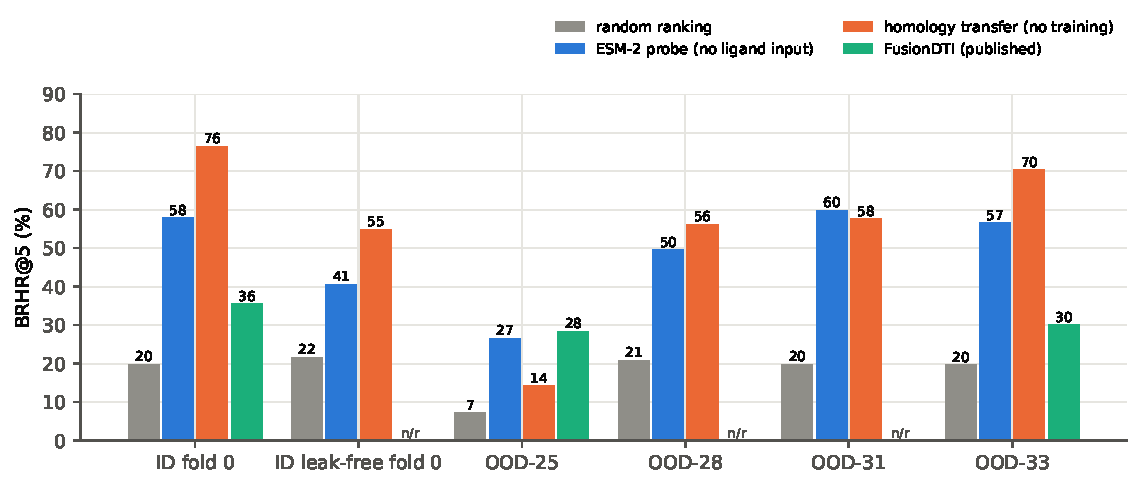
\includegraphics[width=\textwidth]{figures/F4_localization_without_ligand.pdf}
\caption{BRHR@5 by split for random ranking, the ligand-blind ESM-2 probe, training-free homology
transfer and published FusionDTI (n/r: not reported). ID values are means over folds (5 for
FASTA-grouped, 4 for leak-free).}
\label{fig:loc}
\end{figure*}

\subsection{The protein-OOD splits leak}
Table~\ref{tab:leakood} shows, for each OOD split, the share of test pairs whose closest training
protein is more similar than the split allows. The 33\% split leaks under either identity formula:
at least 60.7\% of its test pairs exceed the cap when identity is divided by alignment length, and
67.4\% when it is divided by the shorter sequence. Random test--train pairs exceed the same cap
only 0.5\% of the time. For the 25--31\% splits the verdict depends on the formula, which the
benchmark leaves unstated. Between 3.8 and 29.0\% of pairs exceed the cap under the first
definition, and between 46.2 and 59.5\% under the second. Localization performance follows the
leakage closely (Fig.~\ref{fig:ident}). On the 33\% split, homology-transfer BRHR@1 is 20.2 for
test pairs whose nearest training protein is below 30\% identity and 63.9--67.8 once that identity
exceeds 50\%, while random ranking stays near 4.3.

\begin{table}[t]
\caption{Test pairs (\%) with a training protein above the split's nominal similarity cap.}
\label{tab:leakood}
\centering
\begin{tabular}{lcccc}
\toprule
Split & Local, cov$\geq$0.8 & NW / aln. & NW / shorter & Random pairs \\
\midrule
OOD-25 & 0.0 & 3.8 & 56.6 & 0.0 \\
OOD-28 & 25.0 & 18.0 & 59.5 & 0.0 \\
OOD-31 & 32.4 & 29.0 & 46.2 & 0.1 \\
OOD-33 & 58.2 & 60.7 & 67.4 & 0.5 \\
\bottomrule
\end{tabular}

\\[2pt]
\footnotesize{Local: MMseqs2 identity with alignment covering $\geq80\%$ of the test protein. NW:
global Needleman--Wunsch identity over top-10 candidates (a lower bound), divided by alignment
length or by the shorter length. Random pairs: 1,000 random test--train pairs, NW/aln.}
\end{table}

\begin{figure*}[t]
\centering
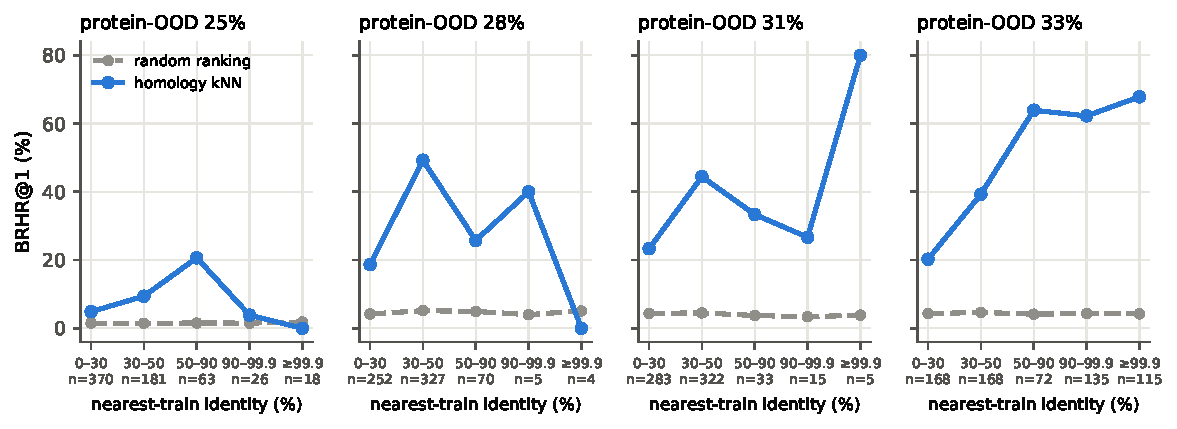
\includegraphics[width=\textwidth]{figures/F2_brhr_by_identity.pdf}
\caption{Homology-transfer BRHR@1 by the test protein's nearest-training identity on the four
protein-OOD splits; $n$ is the number of test pairs per bin.}
\label{fig:ident}
\end{figure*}

\subsection{Standard clustering leaks; a leak-defined split does not}
Table~\ref{tab:leakid} compares the ID splits. Clustering with MMseqs2 at 30\% identity, in either
mode, still leaves 34.0\% of test pairs with a training neighbour of at least 90\% identity over at
least 80\% of the test sequence. The culprit is \texttt{--cov-mode 0}, which demands coverage of
both sequences. A fragment or a single domain therefore never joins the cluster of its full-length
parent, and the two can end up in different folds. Our leak-defined split removes these neighbours
completely. On it, homology transfer drops to 21.7 BRHR@1 and 43.5 BRHR@5. That is still about five
times random, and level with FusionDTI's published ID results. The ligand shortcut does not move at
all (99.7 AUROC), as expected, since the split only constrains proteins.

The signal that survives the leak-defined split is genuine. We examined it on fold~0 of the
connected-component split. Test pairs whose five best homologs all share less than 30\% identity
still reach 41.4 BRHR@1, and 48.8 when the alignment covers at least 80\% of the sequence. Pairs
with no detectable homolog fall to random (2.1), and a prior based only on amino-acid type scores
about 7. Binding-pocket positions are evidently conserved across protein families well below the
30\% identity line that most splitting procedures rely on.

\begin{table}[t]
\caption{ID split variants.}
\label{tab:leakid}
\centering
\resizebox{\columnwidth}{!}{\begin{tabular}{lccccc}
\toprule
ID split & Leak$^f$ & Med. id. & Hom.@1 & Hom.@5 & Bin. AUROC$^g$ \\
\midrule
FASTA-grouped & 75.5 $\pm$ 0.5 & 99.8 $\pm$ 0.0 & 57.5 $\pm$ 0.8 & 77.1 $\pm$ 0.7 & 99.9 $\pm$ 0.0 \\
MMseqs2 30\%, set cover & 34.0 $\pm$ 1.3 & 70.7 $\pm$ 7.8 & 32.7 $\pm$ 2.2 & 55.5 $\pm$ 2.7 & 99.8 $\pm$ 0.0 \\
MMseqs2 30\%, conn. comp. & 34.0 $\pm$ 4.1 & 73.3 $\pm$ 15.0 & 31.4 $\pm$ 2.5 & 53.9 $\pm$ 3.8 & 99.8 $\pm$ 0.0 \\
Leak-defined (ours) & 0.0 $\pm$ 0.0 & 30.9 $\pm$ 0.8 & 21.7 $\pm$ 5.2 & 43.5 $\pm$ 7.8 & 99.7 $\pm$ 0.1 \\
\bottomrule
\end{tabular}
}
\\[2pt]
\footnotesize{$^f$Test pairs (\%) with a training neighbour at $\geq90\%$ identity and $\geq80\%$
coverage. Med.\ id.: median nearest-training identity (\%). Hom.: homology-transfer BRHR.
$^g$Ligand+protein GBM where available, otherwise ligand-only GBM on RDKit descriptors.}
\end{table}

\begin{figure*}[t]
\centering
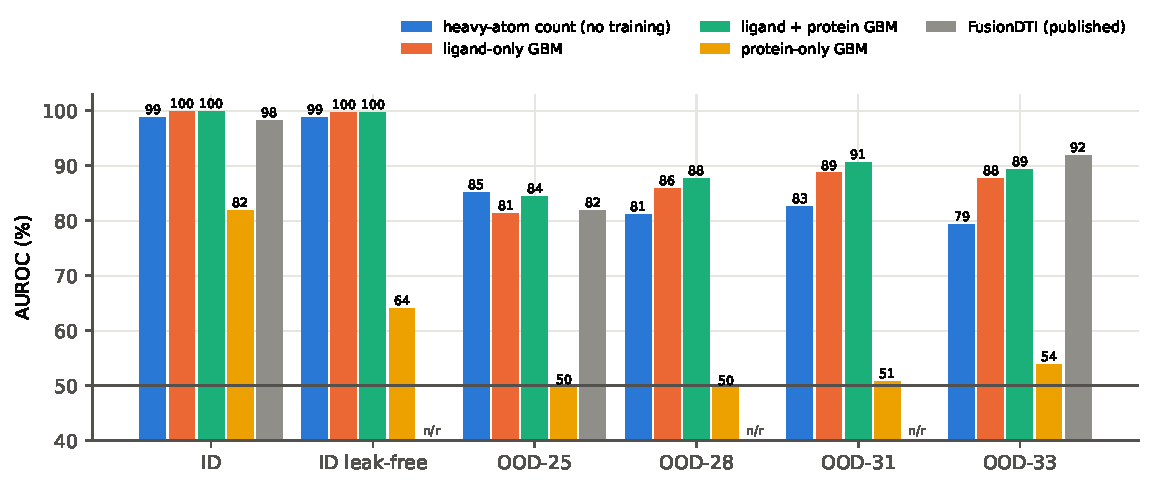
\includegraphics[width=\textwidth]{figures/F3_binary_shortcut.pdf}
\caption{Binary-task AUROC of ligand-size, ligand-only, ligand+protein and protein-only models
against published FusionDTI (n/r: not reported).}
\label{fig:binary}
\end{figure*}

\section{Discussion}
Taken together, the results suggest a few changes to how InteractBind numbers are reported. Every
result should be accompanied by the cheap baselines studied here: a ligand-only model, a
protein-only model, homology transfer and the ligand-agnostic oracle. None of them needs more than
a few minutes on a CPU, and without them a high score cannot be read as evidence of learned
interactions. Localization should be evaluated on protein splits that are built from the leakage
criterion itself, using coverage of either sequence, rather than on \texttt{--cov-mode 0} clusters.
The binary task should also be reported on size-matched subsets, with the caveat that ligand
chemistry beyond size will still carry signal there.

The ligand-specificity results deserve particular attention from anyone building
interaction-aware models. Because the BRHR@5 ceiling for ligand awareness is only 18 points on ID,
BRHR largely measures whether a model finds the pocket, not whether it understands which part of
the pocket a given ligand uses. A model that claims to learn interactions should show a positive
LSG. The binary labels raise a separate issue. Because they are docking thresholds, they encode
ligand size, and they should either be size-corrected or paired with property-matched decoys, as is
already standard practice for docking benchmarks~\cite{dude2012}.

Our study has limitations. We did not retrain any published model, because a single epoch of
DrugBAN~\cite{drugban2023} takes about 100 minutes on our CPU. We can therefore show that the
shortcuts exist and that simple models learn them, but not which shortcuts a particular published
model relies on. Our ID folds also differ from the unreleased originals, so ID comparisons with
published numbers are indicative; the OOD comparisons are direct. The probe uses the smallest ESM-2
model, and we did not test whether larger models change the picture. The global identity values
are lower bounds, because only MMseqs2 candidates were aligned. Finally, LSG can only be computed
for proteins with several annotated test ligands.

\section{Conclusion}
InteractBind's binary task comes close to being a ligand-size test, and models that never see the
ligand meet most of what its localization metric asks for. Its protein-OOD splits, and the 30\%
clustering commonly used to repair such splits, both let homologs through. Until cheap shortcut
baselines and leak-defined splits are part of standard reporting, progress on this benchmark should
not be read as progress in learning drug--target interactions.

\section*{Code and Data Availability}
% TODO: add the public repository URL before submission.
All code, configurations, split files and results are available at [repository URL]. Running
\texttt{make audit} reproduces every number in this paper.

\bibliographystyle{IEEEtran}
\bibliography{refs}

\end{document}
